\documentclass{article}
\usepackage{amsmath}
\usepackage{titlesec}
\usepackage{graphicx}
\usepackage[margin=1in]{geometry}
\usepackage{hyperref}
\usepackage{float}

% Title, date, and author
\title{Exercise 5}
\author{Your Name, Collaborator's Name}
\date{\today}

\titleformat{\section}
  {\normalfont\normalsize\bfseries} % Format: font style, size, and weight
  {\thesection}{1em} % Label format and spacing
  {}
  \renewcommand{\thesubsection}{\thesection.\alph{subsection}}

\titleformat{\subsection}
  {\normalfont\small\bfseries} % Format: font style, size, and weight
  {\thesubsection}{1em} % Label format and spacing
  {}
\titleformat{\subsubsection}
  {\normalfont\small\bfseries} % Format: font style, size, and weight
  {\thesubsubsection}{1em} % Label format and spacing
  {}

\begin{document}
\begin{titlepage}
    \centering
    \vspace*{1in}
    
    {\Huge\bfseries Exercise 5\par}
    \vspace{1.5cm}
    {\Large \today\par}
    \vspace{1.5cm}
    {\Large\itshape Antonio Pampalone 23586519 \\ Giuseppe Pisante 23610012\\ Martina Raffaelli 23616907 \par}
    
    \vfill
    
\includegraphics[width=0.3\textwidth]{FAU-Logo.png}\par\vspace{1cm} % Adjust the width as needed
   
\end{titlepage}

\newpage
\small
\section{Implicit Euler scheme for diffusion equation}
\subsection{Discretization}
Recalling the general form of the implicit Euler method:
\begin{equation*}
  \phi^{n+1}_{i,j} = \phi^{n}_{i,j} + f(\phi^{n+1}, t^{n+1}) \Delta t 
\end{equation*}
we get for the diffusion equation:
\begin{equation*}
  \phi^{n+1}_{i,j} = \phi^{n}_{i,j} + \alpha (\frac{\partial^2 \phi^{n+1}_{i,j}}{\partial x^2} + \frac{\partial^2 \phi^{n+1}_{i,j}}{\partial y^2}) \Delta t
\end{equation*}

Then we use the second order central difference scheme for the spatial derivatives:
\begin{equation*}
  \frac{\partial^2 \phi^{n+1}_{i,j}}{\partial x^2} = \frac{\phi^{n+1}_{i+1,j} - 2\phi^{n+1}_{i,j} + \phi^{n+1}_{i-1,j}}{\Delta x^2}
\end{equation*}
\begin{equation*}
  \frac{\partial^2 \phi^{n+1}_{i,j}}{\partial y^2} = \frac{\phi^{n+1}_{i,j+1} - 2\phi^{n+1}_{i,j} + \phi^{n+1}_{i,j-1}}{\Delta y^2}
\end{equation*}

Substituting the above equations into the diffusion equation, we get:
\begin{equation} \label{discretization}
  \phi^{n+1}_{i,j} = \phi^{n}_{i,j} + \alpha \left( \frac{\phi^{n+1}_{i+1,j} - 2\phi^{n+1}_{i,j} + \phi^{n+1}_{i-1,j}}{\Delta x^2} + \frac{\phi^{n+1}_{i,j+1} - 2\phi^{n+1}_{i,j} + \phi^{n+1}_{i,j-1}}{\Delta y^2} \right) \Delta t
\end{equation}
where we can rearrange the terms to get the following expression:
\begin{equation}
  \phi^{n+1}_{i,j} (1 + 2 \alpha \Delta t(\frac{1}{\Delta x^2} + \frac{1}{\Delta y^2})) - \alpha \Delta t \left( \frac{\phi^{n+1}_{i+1,j} + \phi^{n+1}_{i-1,j}}{\Delta x^2} + \frac{\phi^{n+1}_{i,j+1} + \phi^{n+1}_{i,j-1}}{\Delta y^2} \right) = \phi^{n}_{i,j}
\end{equation}

\subsection{Consistency proof}
In order to prove consistency of the discretization we have to show that the truncation error $T$ goes to zero as the grid spacing ($\Delta x, \Delta y$) goes to zero and the time step ($\Delta t$) goes to zero.


We start with the exact form of the diffusion equation:

\begin{equation}
\frac{\partial \phi}{\partial t} = \alpha \left( \frac{\partial^2 \phi}{\partial x^2} + \frac{\partial^2 \phi}{\partial y^2} \right).
\end{equation}

The discretized scheme for the implicit Euler method is described by equation \eqref{discretization}.

To analyze the truncation error, we expand \( \phi_{i+1,j}^{n+1}, \phi_{i-1,j}^{n+1}, \phi_{i,j+1}^{n+1}, \phi_{i,j-1}^{n+1} \) using Taylor series around \( \phi_{i,j}^{n+1} \). For example, the expansion for \( \phi_{i+1, j}^{n+1} \) is given by:

\begin{equation*}
\phi_{i+1,j}^{n+1} = \phi_{i,j}^{n+1} + \Delta x \frac{\partial \phi}{\partial x} + \frac{\Delta x^2}{2} \frac{\partial^2 \phi}{\partial x^2} + \frac{\Delta x^3}{6} \frac{\partial^3 \phi}{\partial x^3} + \cdots,
\end{equation*}

and similar expansions hold for the other terms. Then we substitute these expansions into the discretized scheme. For example, the term 

\begin{equation*}
\frac{\phi_{i+1, j}^{n+1} - 2\phi_{i,j}^{n+1} + \phi_{i-1,j}^{n+1}}{\Delta x^2}
\end{equation*}

becomes:

\begin{equation*}
\frac{\partial^2 \phi}{\partial x^2} + \frac{\Delta x^2}{12} \frac{\partial^4 \phi}{\partial x^4} + \cdots.
\end{equation*}

Substituting all the Taylor expansions into the discretized equation and rearranging terms, we obtain the residual or truncation error as:

\begin{equation}
T = \Delta t \frac{\partial^2 \phi}{\partial t^2} + \frac{\Delta x^2}{12} \frac{\partial^4 \phi}{\partial x^4} + \frac{\Delta y^2}{12} \frac{\partial^4 \phi}{\partial y^4} + \cdots.
\end{equation}

As \( \Delta t \to 0 \), \( \Delta x \to 0 \), and \( \Delta y \to 0 \), the truncation error \( T \) approaches zero, demonstrating that the discretization is consistent.


\subsection{Stability criteria}

To determine the stability criterion for the implicit Euler scheme using the Von Neumann method, we start with the discretized equation \eqref{discretization} and we
introduce the parameters $ r_x = \frac{\alpha \Delta t}{\Delta x^2} $ and $ r_y = \frac{\alpha \Delta t}{\Delta y^2} $, then the equation becomes:
\begin{equation*}
\phi_{i,j}^{n+1} = \phi_{i,j}^n + r_x \left( \phi_{i+1,j}^{n+1} - 2\phi_{i,j}^{n+1} + \phi_{i-1,j}^{n+1} \right) + r_y \left( \phi_{i,j+1}^{n+1} - 2\phi_{i,j}^{n+1} + \phi_{i,j-1}^{n+1} \right).
\end{equation*}

Rearranging terms, we write:
\begin{equation*}
\phi_{i,j}^{n+1} \left( 1 + 2r_x + 2r_y \right) = \phi_{i,j}^n + r_x \left( \phi_{i+1,j}^{n+1} + \phi_{i-1,j}^{n+1} \right) + r_y \left( \phi_{i,j+1}^{n+1} + \phi_{i,j-1}^{n+1} \right).
\end{equation*}

The Von Neumann method assumes a Fourier mode solution of the form:
\begin{equation*}
\phi_{i,j}^n = G^n e^{I(k_x i \Delta x + k_y j \Delta y)},
\end{equation*}
where $ G $ is the amplification factor,$ k_x $ and $ k_y $ are the wave numbers in the $ x $- and $ y $-directions, and $ I = \sqrt{-1} $.

We substituting this Fourier mode into the discretized equation, and the neighboring terms become:
\begin{equation*}
\phi_{i+1,j}^{n+1} = G e^{I k_x \Delta x} \phi_{i,j}^{n+1}, \quad \phi_{i-1,j}^{n+1} = G e^{-I k_x \Delta x} \phi_{i,j}^{n+1},
\end{equation*}
\begin{equation*}
\phi_{i,j+1}^{n+1} = G e^{I k_y \Delta y} \phi_{i,j}^{n+1}, \quad \phi_{i,j-1}^{n+1} = G e^{-I k_y \Delta y} \phi_{i,j}^{n+1}.
\end{equation*}

Using these expressions, substitute into the equation. Simplify the exponentials using $ e^{I \theta} + e^{-I \theta} = 2 \cos \theta $, leading to:
\begin{equation*}
G \phi_{i,j}^{n+1} \left( 1 + 2r_x + 2r_y \right) = \phi_{i,j}^n + 2r_x G \phi_{i,j}^{n+1} \cos(k_x \Delta x) + 2r_y G \phi_{i,j}^{n+1} \cos(k_y \Delta y).
\end{equation*}

Factoring $G$ from the left-hand side:

\begin{equation*}
G \left( 1 + 2r_x + 2r_y - 2r_x \cos(k_x \Delta x) - 2r_y \cos(k_y \Delta y) \right) = 1.
\end{equation*}

We solve for $ G $:
\begin{equation*}
G = \frac{1}{1 + 2r_x + 2r_y - 2r_x \cos(k_x \Delta x) - 2r_y \cos(k_y \Delta y)}.
\end{equation*}

The scheme is stable if $ |G| \leq 1 $. For the implicit Euler method, the denominator in $ G $ is always greater than 1 for all $ k_x $ and $ k_y $. So we have that:
\begin{equation}
|G| \leq 1,
\end{equation}
which implies unconditional stability.

\subsection{Convergence proof}
Since the scheme is both consistent and stable, for the Lax equivalence theorem, the scheme is convergent.

\section{Finite-volume method}

\subsection{Co-located grid}

In the co-located finite volume method, all variables are stored at the same location, typically the cell center. This approach uses the 
same control volumes for all conservation equations, which minimizes programming and storage effort, especially for geometric quantities. 
It is particularly beneficial in handling complex geometries, as control volumes can easily conform to complicated boundaries. However, 
a significant challenge is the pressure-velocity coupling, which can lead to oscillations in the pressure field. This issue is often 
addressed using "momentum interpolation" to ensure stability. 

\subsection{Staggered grid}

A staggered grid is a numerical technique in which different variables are stored at different locations within the control volume. 
Specifically, pressure is stored at the center of the cell, while velocity components are stored at the faces of the cell. This results in 
different control volumes for different equations. One of the primary advantages of the staggered grid is that many terms can be calculated 
without the need for interpolation, maintaining second-order accuracy. It provides strong coupling between the pressure and velocity fields, 
which helps prevent oscillations in the solution, ensuring stability. However, a significant disadvantage of the staggered grid is the difficulty 
and computational expense of extending it to arbitrary, curvilinear, and non-orthogonal grids, which limits its flexibility in handling complex geometries.

\subsection{Variable arrangements}

In the picture reported below, the staggered variable arrangement is illustrated as (1). In contrast, (2) shows the co-located variable arrangement.

\begin{figure}[h!]
  \centering
  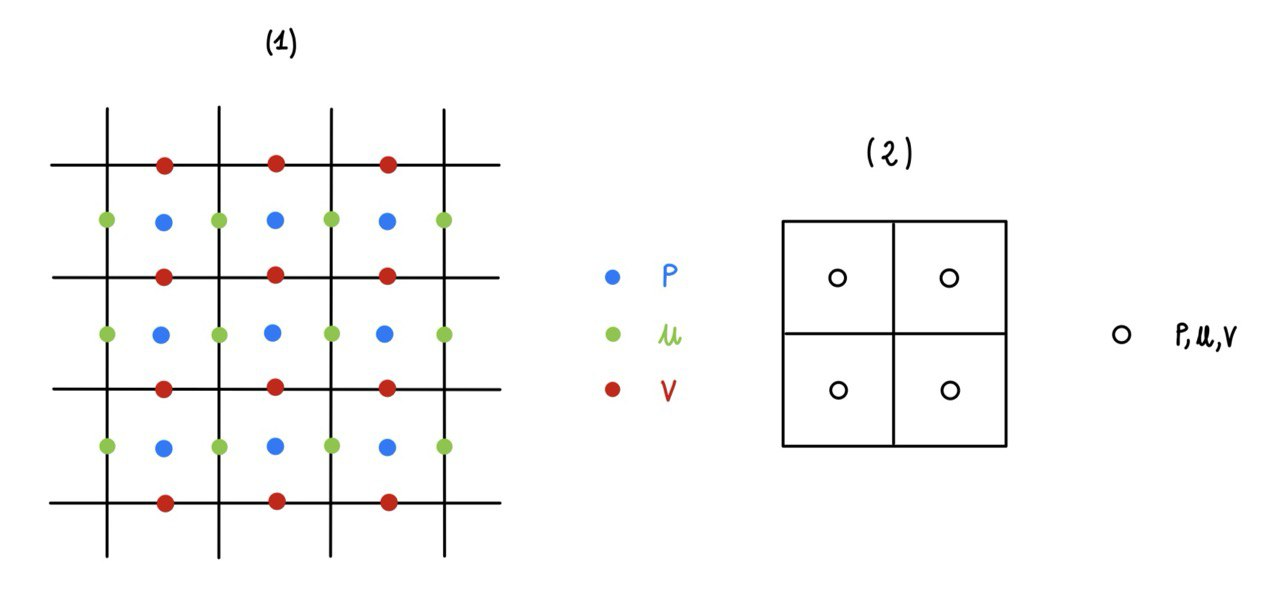
\includegraphics[width=0.5\textwidth]{Variable.jpg}
  \caption{Variable arrangements}
\end{figure}

\subsection{Integral form of the equation}

To derive the integral form of the partial differential equation, we integrate over a control volume:
\[
\int_V \frac{\partial (\rho \Phi)}{\partial t} \, dV + \int_V \nabla \cdot (\rho \vec{u} \Phi - \alpha \nabla \Phi) \, dV = \int_V S_\Phi \, dV
\]
Applying the divergence theorem to the second term, we obtain:
\[
\int_V \frac{\partial (\rho \Phi)}{\partial t} \, dV + \int_{\partial V} (\rho \vec{u} \Phi - \alpha \nabla \Phi) \cdot \vec{n} \, dA = \int_V S_\Phi \, dV
\]

\subsection{Approximation of the volume and surface integral}

Using the mid-point rule, volume integrals over are approximated by evaluating the integrand at the center of the control volume \( P \).
\[
\int_V \frac{\partial (\rho \Phi)}{\partial t} \, dV \approx \frac{\partial (\rho \Phi)_P}{\partial t} \Delta x \Delta y
\]
Surface integrals over are approximated by evaluating fluxes through face at the midpoints of the faces of the control volume.
\[
\int_{\partial V} \left( \rho u \Phi - \alpha \nabla \Phi \right) \cdot n \, dA \approx \sum_f F_f A_f
\]


\subsection{Approximation of the source term and time derivative}

The source term \( S_\Phi \) is assumed constant within the control volume:
\[
\int_V S_\Phi \, dV \approx S_{\Phi, P} \Delta x \Delta y
\]
The time derivative is discretized using a finite difference method. For a first-order explicit scheme:
\[
\frac{\partial (\rho \Phi)_P}{\partial t} \approx 
\frac{(\rho \Phi)_P^{n+1} - (\rho \Phi)_P^n}{\Delta t}
\]

\subsection{Approximation of the Flux terms}

\subsection*{Convective Fluxes}

The upwind scheme uses the value of $\Phi$ from the upstream cell based on the flow direction:
\begin{equation}
(\rho u \Phi)_f = \rho_f u_f \Phi_{\text{upwind}}
\end{equation}
For example at the east face, if $u_e > 0$, $\Phi_{\text{upwind}} = \Phi_P$, so:
\begin{equation}
  (\rho u \Phi)_e = \rho_e u_e \Phi_P 
  \end{equation}
The central scheme uses the average value of $\Phi$ from adjacent cells on either side of the face:
\begin{equation}
(\rho u \Phi)_f = \rho_f u_f \frac{\Phi_L + \Phi_R}{2}
\end{equation}
For example, at the east face, $\Phi_L = \Phi_P$ and $\Phi_R = \Phi_E$, so:
\begin{equation}
(\rho u \Phi)_e = \rho_e u_e \frac{\Phi_P + \Phi_E}{2}
\end{equation}

\subsection*{Diffusive Fluxes}

A central difference scheme is used to approximate the gradient of $\Phi$ at each face:
\begin{equation}
(\nabla \Phi)_f = \frac{\Phi_R - \Phi_L}{\Delta x_f}
\end{equation}
For example, at the east face:
\begin{equation}
(\nabla \Phi)_e = \frac{\Phi_E - \Phi_P}{\Delta x_e}
\end{equation}

\subsection{Final Discretized Equation}

For a uniform grid, the final discretized equation it's given by:

\begin{align*}
\frac{(\rho \Phi)_P^{n+1} - (\rho \Phi)_P^n}{\Delta t} \Delta x \Delta y + \Delta y \Bigg[ & (\rho u \Phi)_e - (\rho u \Phi)_w - \alpha \frac{\Phi_E - \Phi_P}{\Delta x} + \alpha \frac{\Phi_P - \Phi_W}{\Delta x} \Bigg] \\
+ \Delta x \Bigg[ & (\rho v \Phi)_n - (\rho v \Phi)_s - \alpha \frac{\Phi_N - \Phi_P}{\Delta y} + \alpha \frac{\Phi_P - \Phi_S}{\Delta y} \Bigg] = S_{\Phi, P} \Delta x \Delta y
\end{align*}

\subsection{Flux blending}

Flux blending is used to combine the advantages of both schemes. The CDS is second-order accurate in space, providing higher accuracy when the
flow is smooth however, it can cause numerical oscillations, especially in cases with high Peclet numbers. The UDS is first-order 
accurate in space but is stable and avoids oscillations in high Peclet number flows. Flux blending provides the stability of the UDS whith higher 
accuracy of the CDS. The blending ratio $\beta$ allows control over the relative contributions of these two schemes. A good blending ratio can be derived 
based on the Peclet number:
\[
\beta = \frac{Pe}{1 + Pe}
\]
This formula ensures:
\[
\beta \to 0 \quad \text{as} \quad Pe \to 0 \quad \text{(diffusion-dominated)}
\]

\[
\beta \to 1 \quad \text{as} \quad Pe \to \infty \quad \text{(convection-dominated)}
\]

\subsection{Boundary conditions}

At a velocity inlet, a specified velocity boundary condition is given. The mass flux and convective flux are computed using the given velocity 
and other variables such as density and velocity components. To compute the diffusive flux the gradient of the scalar quantities is computed using
one-sided finite differences. At a solid (impermeable) wall, there is no mass flux because the normal velocity component is zero along the wall. 
Similarly, due to zero velocity along the wall, the convective flux is zero as well. In contrast, the diffusive flux inside the momentum equation 
is not equal to zero and contributes to momentum transfer due to shear stress. At a symmetry boundary, the boundary normal velocity component is zero,
so the mass flux through the boundary is equal to zero as weel as the convective flux of all variables is equal to zero. The diffusive fluxes
of all scalar quantities is also equal to zero since the scalar gradients normal to the symmetry boundary are zero.

\subsection{Advantages of a fully coupled and a sequential solution of NSE}

A fully coupled sequential solution of the Navier-Stokes equations involves solving the equations step by step, with feedback between the 
pressure and velocity fields at each time step. The advantage of this approach is that coupling ensures that the pressure and velocity fields
are adjusted iteratively to maintain physical consistency, which can improve stability compared to uncoupled methods where only individual 
variables are solved separately.


\begin{thebibliography}{9}
  \bibitem{GitHubRepo}
  \textit{CFD Repository},\\
  Available at: \url{https://github.com/GiuseppePisante/CFD.git}
  
  \bibitem{GitHubCopilot}
  \textit{GitHub Copilot},\\
  GitHub. Available at: \url{https://github.com/features/copilot}
  
\end{thebibliography}

\end{document}